\documentclass{report}

\usepackage[T1]{fontenc}
\usepackage{titlesec}
\usepackage{amsmath}
\usepackage{amssymb}
\usepackage{xfrac}
\usepackage{todonotes}
\usepackage{array}
\usepackage{tikz}
\usepackage{pgfplots}
\usepackage{tabularx}
\usepackage{subcaption}
\usepackage{graphicx}
\graphicspath{{images/}}
%\pgfplotsset{compat=1.14}
\addtolength{\oddsidemargin}{-.875in}
\addtolength{\evensidemargin}{-.875in}
\addtolength{\textwidth}{1.75in}
\addtolength{\topmargin}{-.875in}
\addtolength{\textheight}{1.75in}

\titleformat{\chapter}{\normalfont\huge}{\thechapter.}{30pt}{\huge}

\newcolumntype{M}[1]{>{\centering\arraybackslash}m{#1}}

\title{Bioengineering Imaging Track Qualifying Exam Study Book}
\author{Markus Foote and Blake Zimmerman}

\begin{document}
	\maketitle
	\setcounter{tocdepth}{1} % Only include down to sections, not subsections
	\tableofcontents
	\part{Finished}
	\chapter{Affine Transform}
	\section{General Transformation Concept}

An \emph{affine transform} is the combination of a \underline{linear} transformation with a \underline{translation}. In a linear algebra context, a point in space is a column vector of individual values along each dimension, i.e. $\left[\begin{matrix}x\\y\end{matrix}\right]$ or $\left[\begin{matrix}x\\y\\z\end{matrix}\right]$ in 2 or 3 dimensions, respectively. This location is noted simply as $\vec{x}$.

The affine transform can thus be written as a matrix-vector multiplication, followed by vector addition:
\begin{equation}
\vec{y} = \mathbf{A}\vec{x} + \vec{b}
\end{equation}

The linear transformation matrix $\mathbf{A}$ has some important special cases and properties:
\begin{description}
	\item[Scaling] This transformation scales each direction of a vector space by the corresponding $c$ value: $$\mathbf{A}=\left[\begin{matrix}
	c_x & 0 \\ 0 & c_y
	\end{matrix}\right] \text{ or } \left[\begin{matrix}
	c_x & 0 &0\\ 0 & c_y &0\\ 0&0&c_z
	\end{matrix}\right]$$
	
	\item[Rotation] This transformation rotates by an angle $\theta$ about the origin in 2 dimensions:$$\mathbf{A}=\left[\begin{matrix}
	\cos(\theta) & -\sin(\theta) \\\sin(\theta) & \cos(\theta)
	\end{matrix}\right]$$ 

	\item[Identity/Translation] This only translates all the points by a constant amount:$$\mathbf{A}=\left[\begin{matrix}
	1 & 0 \\0 &1
	\end{matrix}\right] \text{ and } b=\left[\begin{matrix}t_x\\t_y\end{matrix}\right]$$
	
	\item[Shearing]
	$$\mathbf{A}=\left[\begin{matrix}
	1 & c_x \\c_y &1
	\end{matrix}\right]$$
	\item[In General] $A\in \operatorname{GL}\left(n\right)$ which is the General Linear Group, which means that $A$ has nonzero determinant, and is thus invertible.
	
\end{description}

\section{The Imperfect World}

These transformations are all well and good, but with them so far we can only take points and apply some fun tricks to move them around in cute ways. What if there were \underline{pairs} of points with \emph{known} (or \emph{assumed}) correspondence, and we want to find an affine transform that makes the point pairs \underline{match}?

Using notation:
\begin{align}
\vec{x}_i &\; &\text{source point(s)}\\
\vec{y}_i & &\text{target point(s)}\\
n && \text{total number of point pairs}\\
\mathbf{\mathbf{A}}& & \text{linear transform matrix}\\
T & &\text{translation vector}
\end{align}

In a perfect world, all the points match exactly after being transformed, such that 
\begin{equation}
\vec{y}_i = \mathbf{A} \vec{x}_i +T
\end{equation}
is satisfied. This linear system of equations could be easily solved with some linear algebra.

However, this world is not perfect. Due to noise, human error, systematic error, and spilling coffee on samples before \emph{carefully} wiping it up, there will be noise and the points will not exactly match. There will be some error. We must account for this error.

We want to estimate the best transformation given some number of point pairs that will not all match exactly. Thus, we should minimize the error in the matching using a euclidean distance for the error, and squared error so that this function is convex (which is important when very close to zero error):
\begin{equation}
\underset{\mathbf{A},T}{\min}\sum_i\left\|(\mathbf{A}\vec{x}_i + T) - \vec{y}_i\right\|^2
\end{equation}

\section{Estimating a Solution}

First, if we are given $\mathbf{A}$, then 
\begin{equation}
\delta T = 2 \sum_i^n \left(\mathbf{A}\vec{x}_i + T-\vec{y}_i\right) = 0
\end{equation}
The variation of T is set to zero because the first derivative of a function is zero at a minimum.
Solving for $T$:
\begin{equation}
T=\frac{1}{n}\sum_{i=1}^n \left(\vec{y}_i-\mathbf{A}\vec{x}_i\right)
\end{equation}
This translation is simply the difference of the centroids of the source and target points. Let us define
\begin{align}
\tilde{y}_i &= \vec{y}_i - \vec{c}_y\\
\tilde{x}_i &= \vec{x}_i - \vec{c}_x
\end{align}
where $c_x$ and $c_y$ are the centroids of each point set. This modification of the problem implicitly removes $T$ since both point sets will have the same centroid (the origin).

Assuming the points are centered the problem
\begin{equation}
\underset{\mathbf{A}}{\min}\sum_i\left\|\mathbf{A}\left(\vec{x}_i-\frac{1}{n}\sum_j \vec{x}_j\right) - \left(\vec{y}_i-\frac{1}{n}\sum_j \vec{y}_j\right)\right\|^2
\end{equation}
simplifies to
\begin{equation}
E = \underset{\mathbf{A}}{\min}\sum_i\left\|\mathbf{A}\tilde{x}_i - \tilde{y}_i\right\|^2 
\end{equation}
Similar to the procedure performed to find and remove $T$, we now find the variation of $\mathbf{A}$ and set it equal to zero:
\begin{equation}
\frac{\partial}{\partial\mathbf{A}} = 2 \sum_i \left(\mathbf{A}\tilde{x}_i-\tilde{y}_i\right)\, \tilde{x}_i^T = 0
\end{equation}
Then solving for $\mathbf{A}$:
\begin{equation}
\mathbf{A}=\left(\sum_i\tilde{y}_i\tilde{x}_i^T\right)\left(\sum_i\tilde{x}_i\tilde{x}_i^T\right)^{-1}
\end{equation}

A special note here about the matrix $\sum_i\tilde{x}_i\tilde{x}_i^T$: A minimum of 3 non-co-linear points in 2D (or 4 non-coplanar points in 3D) are required for this matrix to be invertible. In general, to guarantee that a solution exists for $A$, you need $n+1$ points.


	
	\chapter{Magnetic Resonance Imaging}
	\section{Overview} %TODO Maybe remove this
\textbf{Magnetic Resonance Imaging} (\textbf{MRI}) is an imaging modality that expoits the phenomenon of Nuclear Magnetic Resonance to record information about the local chemical environment of specific atoms within a body. Commonly, these atoms are the hydrogen nuclei, but MRI is possible with any nuclei with a non-integer nuclear spin. Generally, the proceedure for MRI is summarized in the following steps, where only step \ref{item:mri:gensteps:gradients} is specific to the Imaging modality over an NMR experiment:
\begin{enumerate}
	\item \label{item:mri:gensteps:b0} Nuclei align with an applied, strong magnetic field $\vec{B}_0$.
	\item \label{item:mri:gensteps:rf} Radio Frequency energy is applied to flip the nuclear magnetization off-axis from $\vec{B}_0$.
	\item \label{item:mri:gensteps:precess} Interaction between $\vec{B}_0$ and nuclear magnetizations causes magnetizations to \textbf{\textit{precess}}.
	\item \label{item:mri:gensteps:record} Induced current from precessing magnetization is observed in an RF coil.
	\item \label{item:mri:gensteps:gradients} Speed of precession is spatially varied by a spatially-varying magnetic field gradient.
\end{enumerate}
\section{Magnetism and Nuclear Magnetic Resonance}
Magnetism is an inherent property of matter which causes materials to interact with external magnetic fields to generate their own magnetic field. This phenomenon is characterized by the relation
\begin{equation}
\vec{H} = \chi \vec{B} \label{eq:mri:magneticsusceptibility}
\end{equation}
where $\vec{H}$ is the generated field, $\vec{B}$ is the applied field, and $\chi$ is the \textit{magnetic susceptibility} of the matter. Matter is classified into three main categories based on $\chi$:
\begin{description}
	\item[Paramagnetic] matter has \textit{positive} $\chi$, thus $\vec{H}$ points in the same direction as $\vec{B}$. \textbf{Ex:} Aluminum
	\item[Diamagnetic] matter has \textit{negative} $\chi$, thus $\vec{H}$ points in the opposite direction as $\vec{B}$. \textbf{Ex:} Water
	\item[Ferromagnetic] matter has \textit{large} $\chi$. \textbf{Ex:} Iron
\end{description}
Magnetism originates from the electrons of an atom, but Nuclear Magnetic Resonance originates from the nucleus and is still subject to electronic magnetism, or \textit{chemical shift} phenomena.

Nuclear Magnetism arises from nuclei of atoms with odd-even pairing of neutrons and protons, resulting in nuclei with non-integer spin. E.g. $^1$H with spin $I=\sfrac{1}{2}$. Nuclear spin in motion gives rise to an angular momentum of the spin:
\begin{equation}
J=\hbar I = \frac{h}{2\pi}I
\end{equation}
where J is the resulting angular momenta, $h$ is Planck's constant, and $\hbar$ is the reduced Planck constant. 
The magnetic moment of matter is also determined by
\begin{equation}
\mu = \gamma J = \gamma \hbar I
\end{equation}
where $\mu$ is the magnetic moment and $\gamma$ is the \textit{gyromagnetic ratio} that is specific to the nucleus in question.

Bulk magnetization (the collective net magnetization from a region of matter) is dependent upon the relative number of individual moments in the `up' (parallel to $\vec{B}_0$) and `down' (anti-parallel to $\vec{B}_0$) states:
\begin{equation}
\vec{m} = \mu (\Delta N)
\end{equation}
where $N$ is the number of magnetic moments in the up and down states such that $\Delta N$ is the net difference of moments in the anti-parallel direction.
$N$ follows a Boltzmann distribution based on the energy state, $E$, of the nuclei:
\begin{equation}
N\propto e^{-\frac{E}{kT}}
\end{equation}
where $k$ is the Boltzman constant and $T$ is the absolute temperature. The energy state of a magnetic moment is
\begin{equation}
E(\mu) = -\mu B_0 = -\gamma \hbar m B_0
\end{equation}
where $m = \left\{I \ldots\sfrac{3}{2}, \sfrac{1}{2}, -\sfrac{1}{2}, -\sfrac{3}{2},\ldots -I\right\}$ are the permissible states for the spin $I$. Again assuming $^1$H nuclei, the two energy states are
\begin{align}
E\left(\text{up}\right) &= - \gamma \hbar \left(\sfrac{1}{2}\right) B_0 \\
E\left(\text{down}\right) &= + \gamma \hbar \left(\sfrac{1}{2}\right) B_0 .
\end{align}
The ratio of spin alignment can then be calculated:
\begin{equation}
\frac{N\left(\text{up}\right)}{N\left(\text{down}\right)} = e^{+ \frac{\Delta E}{kT}} \label{eq:mri:ratio}
\end{equation}
where $\Delta E = E\left(\text{down}\right) - E\left(\text{up}\right)$. If we then suppose that there exist a total of $N$ nuclei such that $N\left(\text{up}\right) + N\left(\text{down}\right) = N$, then from this and (\ref{eq:mri:ratio}) we can solve for $\Delta N$ and thus $M$:
\begin{equation}
M=\mu \Delta N = \frac{N\gamma^2 \hbar^2 B_0}{4kT}
\end{equation}
This equation can be massaged to match the form of (\ref{eq:mri:magneticsusceptibility}):
\begin{align}
M = \chi_{_0} B_0 && \chi_{_0} = \frac{N\gamma^2 \hbar^2 }{4kT}
\end{align}
where $\chi_{_0}$ is a matter-specific term that describes the resulting magnetic field from an applied field $B_0$. This $\chi_{_0}$ is very small, and results in a very low effective signal from a body of matter. However, there are engineering decisions in each of these terms that helps raise the signal:
\begin{description}
	\item[$\mathbf{B_0}$] Make it big, but not too big. Like 1.5 T at least, probably 7 T is awesome.
	\item[$\mathbf{N}$] Effectively this is the voxel size. Cubic power. $\sfrac{1}{2}$ resolution $\to$ 8x larger voxel $\to$ 64x signal.
	\item[$\mathbf{T}$] Very limited range if you want the subject to be alive, but colder is better.
	\item{$\!\!\mathbf{\gamma}\;$} Pick nuclei with high $\gamma$, and isotope with high abundance. See Table \ref{tab:mri:nuclist}.
\end{description}
\begin{table}[h]
	\caption{\label{tab:mri:nuclist} Relevant Properties of Some Common Nuclei}
	\centering
	\begin{tabular}{|c|c|c|c|}
		\hline Nuclei & $I$ & $\frac{\gamma}{2\pi}$ (MHz/T) & nat. abundance (\%) \\ 
		\hline $^1$H & \sfrac{1}{2} & \textbf{42.58} & 99.98 \\ 
		\hline $^{13}$C & \sfrac{1}{2} & 10.71 & 1.11 \\ 
		\hline $^{19}$F & \sfrac{1}{2} & 40.05 & 100 \\ 
		\hline $^{31}$P & \sfrac{1}{2} & 17.23 & 100 \\ 
		\hline $^{23}$Na & \sfrac{3}{2} & 11.26 & 100 \\ 
		\hline 
	\end{tabular} 
\end{table}

\section{Spin Motion and the NMR Signal}
Precession of the nuclear magnetization, or `spin' is described by
\begin{equation}
\frac{d\vec{m}}{dt}=\gamma \vec{m} \times \vec{B}.
\end{equation}
The resulting motion is analogous to a spinning gyroscope: the rotation does not change, but the \textit{axis of rotation} changes. The precession of earth leads to changes in the classification of the north star, while the typical spinning of earth manifests as day/night.

There are four important cases of spin motion in the context of MRI/NMR:
\begin{enumerate}
	\item First is the case when $\vec{m}$ is aligned with $\vec{B}$, for example $\vec{m} = m_0\; \hat{z}$ and $\vec{B}  = B_0\; \hat{z}$. This results in the derivative term being zero from properties of the vector cross product. This case is stable (see Fig. \ref{fig:mri:stable}).

\item \label{item:mri:precession}The second case is substantially more interesting. If we let 
\begin{equation}
\vec{m} = m_0\; \hat{x}
\end{equation} and \begin{equation}
\vec{B}  = B_0\; \hat{z} ,
\end{equation} then \begin{equation}
 \frac{d\vec{m}}{dt} = - m_0B_0\;\hat{y}\; .
 \end{equation} 
This results in the infinitesimal motion of the magnetization to move in the $-\hat{y}$ direction. As time progresses, the magnetization precesses \textit{about} $-\hat{z}$ at the rate $\omega = -\gamma B_0$, known as the \textit{Larmor} frequency (see Fig. \ref{fig:mri:precession}).
\item Similar to case \ref{item:mri:precession}, the precession about $-\hat{z}$ is stable at any angle $\alpha$ (see Fig. \ref{fig:mri:decay}).

\item Finally, the case of `flipping' the magnetization from alignment with $\hat{z}$ to alignment with $\hat{x}$. Starting with \begin{equation}
\vec{m} = m_0\; \hat{z}
\end{equation} the application of an infinitely short magnetic field pointing in the $-\hat{y}$ direction 
\begin{equation}
\vec{B} = -\delta(t)B_1\hat{y}
\end{equation}results in changing the direction of $\vec{m}$ towards the $\hat{x}$ axis. Realistically, this applied field cannot be infinitely short, so after every bit of time, the $\vec{B}_1$ field must be updated to still be perpendicular to $\vec{m}$. This results in a field applied according to
\begin{equation}
\vec{B}=B_1\big(\cos\left(\omega_0 t\right) - \sin\left(\omega_0 t\right)\big)
\end{equation}
giving a clockwise spin of the applied magnetic field (precession about the $-\hat{z}$ axis). This results in $\vec{m}$ precessing about the $\hat{z}$ axis while being progressively `flipped' to the transverse ($\hat{x}$-$\hat{y}$) plane. The overall `flip' procedure is parameterized by $\alpha$, the resulting angle that $\vec{m}$ makes with the $+\hat{z}$ axis (see Fig. \ref{fig:mri:flip}).

\end{enumerate}

\begin{figure}[h]
	\centering
	\begin{subfigure}[b]{0.22\textwidth}
		\centering
		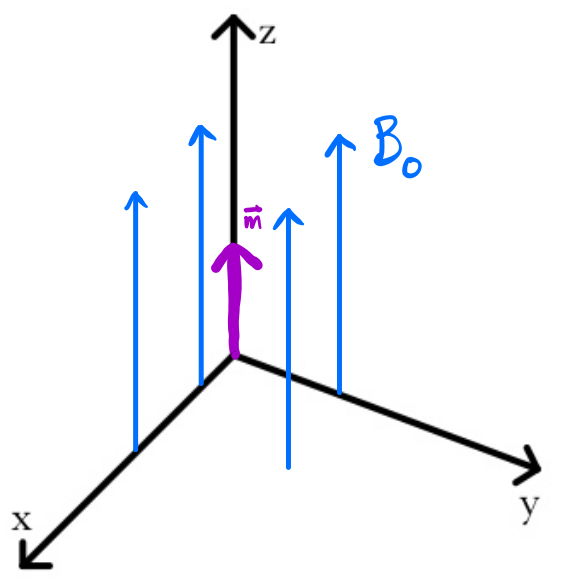
\includegraphics[width=\linewidth]{mri-a}
		\caption{Stable Magnetization}
		\label{fig:mri:stable}
	\end{subfigure}\hfill
	\begin{subfigure}[b]{0.22\textwidth}
		\centering
		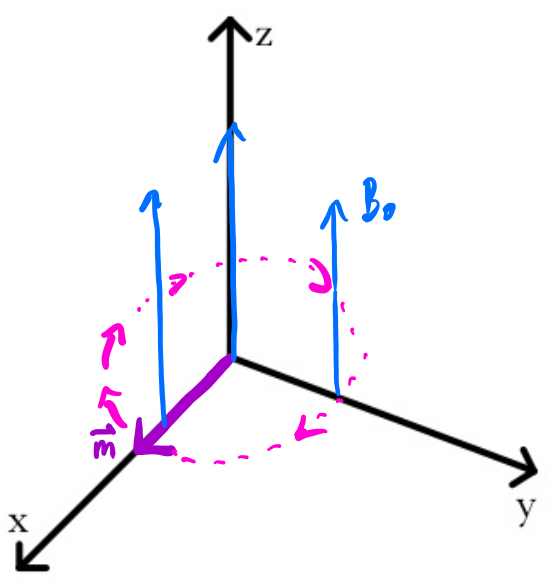
\includegraphics[width=\linewidth]{mri-b}
		\caption{Spin Motion}
		\label{fig:mri:precession}
	\end{subfigure}\hfill
	\begin{subfigure}[b]{0.22\textwidth}
		\centering
		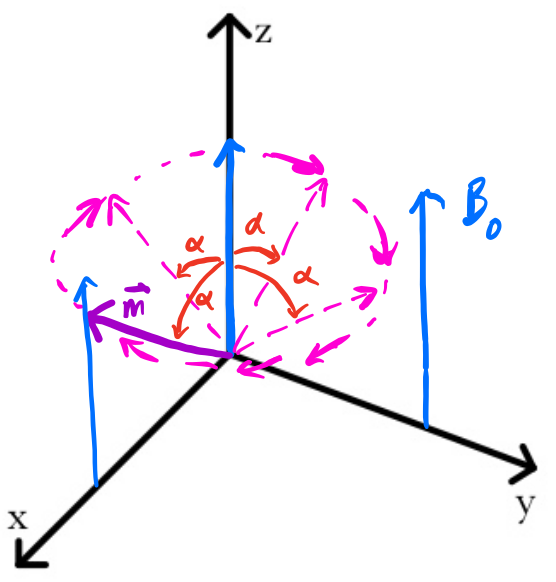
\includegraphics[width=\linewidth]{mri-c}
		\caption{Precession at an angle}
		\label{fig:mri:decay}
	\end{subfigure}\hfill
	\begin{subfigure}[b]{0.22\textwidth}
		\centering
		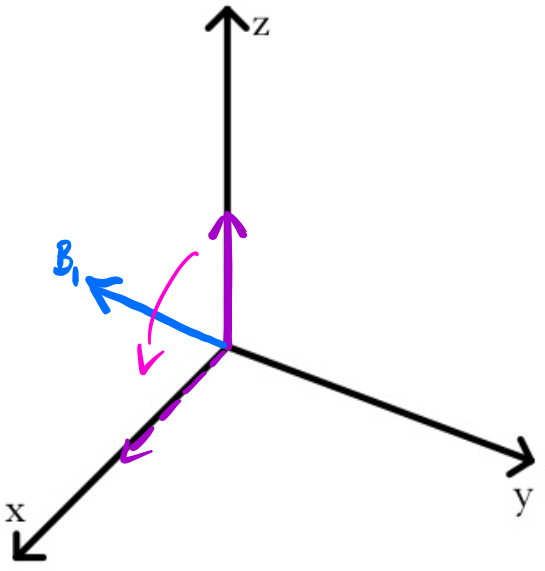
\includegraphics[width=\linewidth]{mri-d}
		\caption{Excitation}
		\label{fig:mri:flip}
	\end{subfigure}
	\caption{Canonical Cases of Spin Motion}\label{fig:mri:cases}
\end{figure}

The fundamentals presented thus far are sufficient to describe the most basic NMR experiment:\\
{\centering
	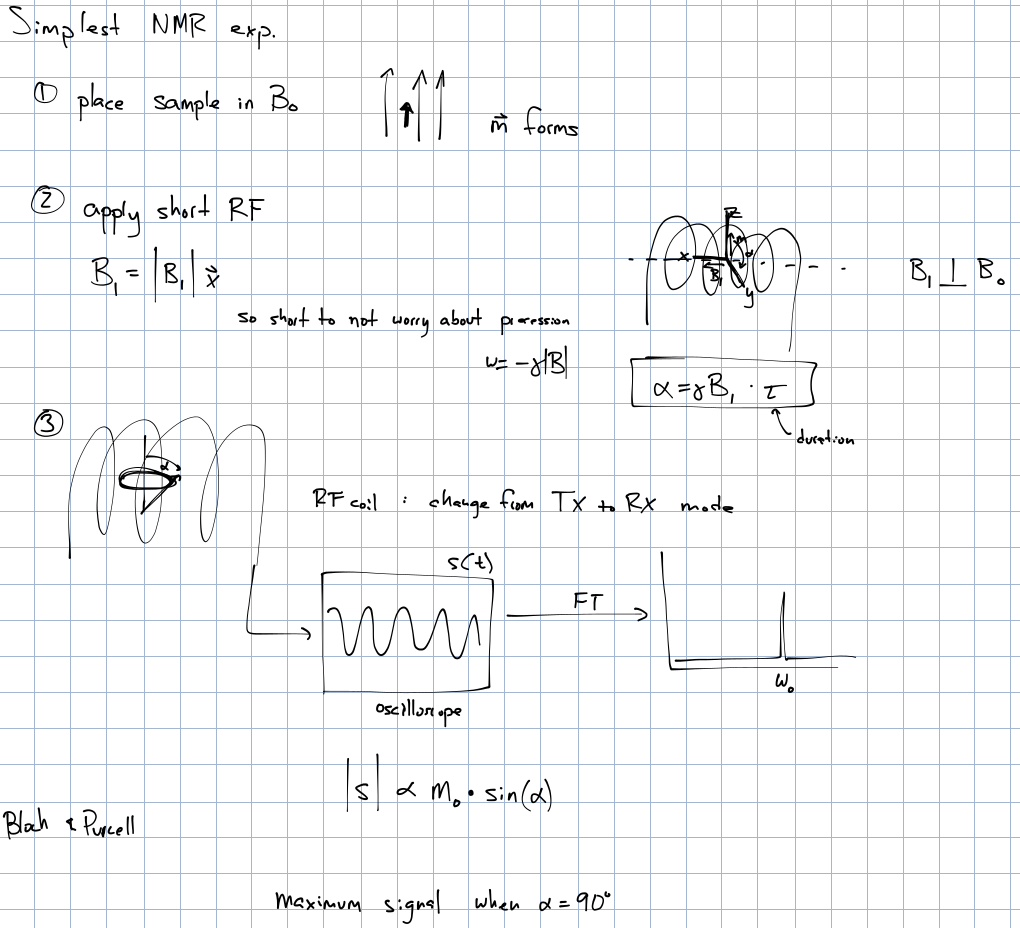
\includegraphics[width=0.8\linewidth]{mri-nmr}
}

\section{Spatial Encoding}
Magnetic Resonance \textit{Imaging} is made possible by encoding spatial information in the NMR signal. This is accomplished by making $B$ a linear function of space using \textit{gradient fields}. These magnetic gradient fields are always parallel to the main $B_0$ field. By changing the magnitude of the magnetic field, the spins precess faster or slower to form a frequency histogram, which is a projection of the object. Example gradient fields are shown in Fig. \ref{fig:mri:gradients}.

\begin{figure}[h]
	\centering
	\begin{subfigure}[b]{0.3\textwidth}
		\centering
		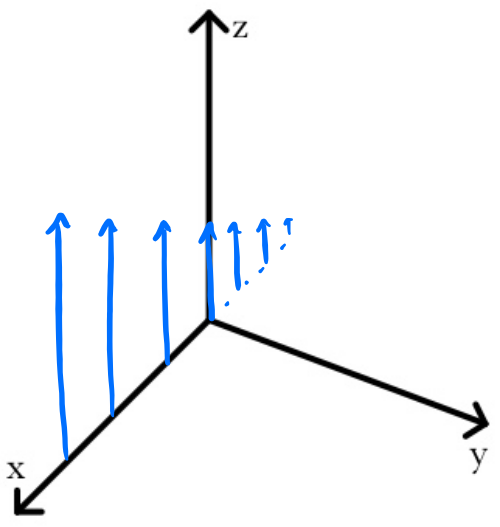
\includegraphics[width=\linewidth]{mri-gradx}
		\caption{$G_x$}
		\label{fig:mri:gradx}
	\end{subfigure}\hfill
	\begin{subfigure}[b]{0.3\textwidth}
		\centering
		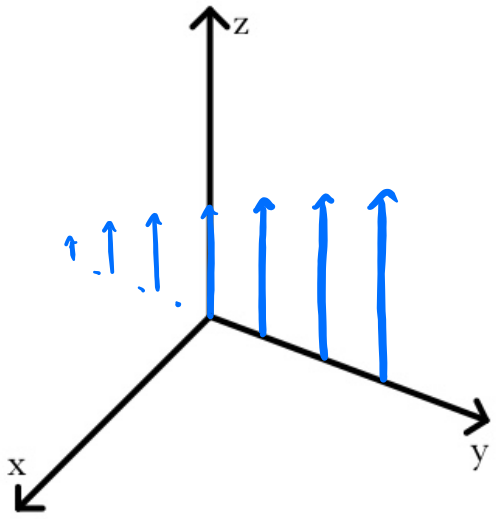
\includegraphics[width=\linewidth]{mri-grady}
		\caption{$G_y$}
		\label{fig:mri:grady}
	\end{subfigure}\hfill
	\begin{subfigure}[b]{0.3\textwidth}
		\centering
		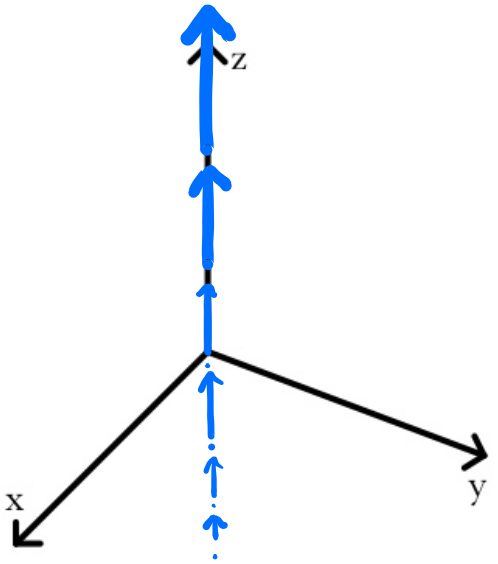
\includegraphics[width=\linewidth]{mri-gradz}
		\caption{$G_z$}
		\label{fig:mri:gradz}
	\end{subfigure}
	\caption{Gradient Fields}\label{fig:mri:gradients}
\end{figure} 

The Larmor frequency is thus dependent on the location of the spin:
\begin{align}
\vec{G} &= \left[\begin{matrix}G_x\\G_y\\G_z\end{matrix}\right]\\
\vec{r} &= \left[\begin{matrix}x\\y\\z\end{matrix}\right]\\
B &= B_0 + \vec{G}\cdot \vec{r}\\
\omega(\vec{r}) &= -\gamma B = -\gamma\left(B_0 + \vec{G}\cdot \vec{r}\right) \label{eq:mri:larmorgrad}
\end{align}
Using this relation and assuming that $m(x,y,z) = m(\vec{r})$ is the proton density image, each magnetization in space will precess at the frequency corresponding to its location by \ref{eq:mri:larmorgrad}. The signal radiated by a single point is 
\begin{equation}
m(\vec{r})e^{i\omega(\vec{r})t}.
\end{equation}
The total signal recorded by a coil surrounding the body is found by integrating over the entire volume:
\begin{equation}
s(t) = \iiint_{\Omega}m(\vec{r})e^{-i\gamma \vec{G}\cdot\vec{r}t}d\vec{r}
\end{equation}
A useful substitution is made by introducing the variable $k$:
\begin{equation}
\vec{k} = \frac{\gamma}{2\pi} \vec{G}t
\end{equation}
\begin{equation}
s(\vec{k}) = \iiint_{\Omega}m(\vec{r})e^{-i2\pi \vec{k}\cdot\vec{r}}d\vec{r}
\end{equation}

Close inspection of this equation reveals that it is simply the forward Fourier Transform of the function of spatial magnetization $m(\vec{r})$. The original magnetization image can be easily obtained by the \textit{inverse} Fourier Transform of the acquired signal.
\section{Slice Selection}
Spatial encoding of the Larmor frequency via gradient fields also enables selective excitation. The target nuclei within the 2D plane (or slab) we aim to excite are provisioned a common resonant frequency by applying a gradient in the direction orthogonal to that plane. The target slice can then be excited by delivering radiofrequency energy at the appropriate frequency via a modulated radiofrequency pulse, especially a sinc-modulated sinusoid. 


\section{MRI Contrast Mechanisms}
\subsection{Spin Lattice Relaxation - T1}
\begin{equation}
\frac{dm_z}{dt}= \frac{m_0-m_z}{T_1}
\end{equation}

\begin{equation}
m_z(t) = \underset{\text{initial condition}}{\underbrace{\qquad\qquad}} e^{\frac{-t}{T_1}} + \underset{\text{final condition}}{\underbrace{\quad m_0\quad}}\left(1-e^{\frac{-t}{T_1}}\right)
\end{equation}

add graph here


\subsection{Spin-Spin Relaxation - T2}
\begin{equation}
T_2 << T_1
\end{equation}

\begin{equation}
\frac{dm_{xy}}{dt}= \frac{-1}{T_1}m_{xy}
\end{equation}

\begin{equation}
m_{xy}(t) = \underset{\text{initial condition}}{\underbrace{\qquad\qquad}} e^{\frac{-t}{T_2}}
\end{equation}

add graph here

\subsection{Dephasing - T2*}
Same as $T_2$, just faster, due to $B_0$ inhomogeneity, spins dephase in $xy$ plane.
\subsection{Bloch Equation}
The $T_1$ and $T_2$ contrast mechanisms are incorporated together in the spin motion equation to fully describe the motion of a nuclear spin through time. In pieces, the equations are the same as what was introduced above in each section.
\begin{align}
\frac{d\vec{m}}{dt} &= \gamma \vec{m} \times \vec{B}  \\
\frac{dm_z}{dt}&= \frac{m_0-m_z}{T_1} =\frac{m_z-m_0}{T_1} \\
\frac{dm_{x}}{dt}&= \frac{-m_{x}}{T_1}  \\
\frac{dm_{y}}{dt}&= \frac{-m_{y}}{T_1}
\end{align}
These equations are written together as a single vector equation:
\begin{equation}
\frac{d\vec{m}}{dt} = \gamma \vec{m} \times \vec{B} -\left[\begin{matrix}\sfrac{1}{T_2}&0&0\\0&\sfrac{1}{T_2}&0\\0&0&\sfrac{1}{T_1}\end{matrix}\right] \left(\vec{m}-\vec{m}_0\right)
\end{equation}
\subsection{Diffusion}
\subsection{FatSat}
	
	\chapter{Image Processing: Hough Transform}
	In image processing the \textbf{Hough Transform} is useful for \textit{global} filtering, especially to find sets of pixels that lie along curves of a specified shape, i.e. finding lines, circles, ellipses, spheres, hypercubes, etc. It provides an elegant solution using a \textit{discretized parameter space}, while the na\"ive, brute-force approach quickly becomes daunting. In the case of finding lines in an image of $n$ points, the na\"ive approach involves iteration over all $\sim\!\! n^2$ possible lines and performing $\sim\!\! n^3$ comparisons for every point to each line. The $O(n^3)$  complexity exponentially worsens for shapes with higher dimensional parameter spaces. This approach is computationally prohibitive for non-trivial applications.

Instead, the Hough Transform accumulates non-background points in a discretized parameter space. The dimensionality of the parameter space is equal to the number of the parameters that describe the desired shape. In the case of a line, there are two parameters. However, the parameters must be defined with care. The na\"ive parameter choices for a line might be \textit{slope} and \textit{intercept}, but if the objective might include finding vertical (or nearly vertical) lines, a method to accurately discretize/store infinity (or very large values) would be required. A better approach is to parameterize lines by their \textit{normal} representation:
\begin{equation}
x \cos (\theta) + y \sin(\theta) = \rho \; . \label{eq:hough:line}
\end{equation}
In this parameterization, all parameters are nicely bounded: $-\sfrac{\pi}{2} \leq \theta \leq \sfrac{\pi}{2}$ and $-D\leq \rho \leq D$ for an image with D length between the two most distant corners.

The Hough Transform is a general algorithm, though in some cases it is analogous to formal mathematical transforms (eg. the Hough transform of lines with 'normal' parameterization is analogous to the Radon Transform). A typical pre-processing step for the image in question is edge detection to form a binary image, though this is not strictly necessary. The algorithm proceeds as follows:
\begin{enumerate}
	\item \label{item:houghalg:allocate} Allocate an accumulator image, selecting the appropriate number and width of bins for each parameter. 
	\item \label{item:houghalg:selectpixel} Select a foreground pixel.
	\item \label{item:houghalg:selectparam} Select center-of-bin values for (the same) $n-1$ of the $n$ parameters.
	\item \label{item:houghalg:solve} Solve for the final parameter value to satisfy the reference equation at the selected pixel.
	\item \label{item:houghalg:increment} Increment the accumulator image at the chosen- and solved- parameter location.
	\item \label{item:houghalg:iterparam} Repeat steps \ref{item:houghalg:selectparam} - \ref{item:houghalg:increment} for all possible chosen parameter values.
	\item \label{item:houghalg:iterpixel} Repeat steps \ref{item:houghalg:selectpixel} - \ref{item:houghalg:iterparam} for all foreground pixels in the image.
	\item \label{item:houghalg:findfeatures} Find parameters for prominent features by the location of accumulator maximum, or thresholding.
\end{enumerate}
In the case of non-binary images, the accumulator simply need not be discrete, such that foreground (or all) pixels just have a partial-voting effect. This algorithm simply extends to higher dimensional images, and higher dimensional parameter spaces. In general, the complexity depends on the number of foreground pixels and the number of parameters; the complexity \textit{increases} by $O(A^{m-2})$ with each additional parameter, where $A$ is the size of the image space, and $m$ is the number of parameters.

As a concrete example, consider the binary image (with foreground as black)
\begin{center}
	\begin{tikzpicture}
\begin{axis}[title=Image, axis equal image, y dir=reverse, enlargelimits=false, tick style={draw=none}]
\addplot[patch,patch type=rectangle, color=black, faceted color=none]
coordinates {
	(0,0) (1,0) (1,1) (0,1) 
	(101, 101) (101,100) (100, 100) (100, 101)
	(101,0) (100,0) (100,1) (101,1)
	(0,101) (1,101) (1,100) (0,100) 
	(51,51) (51,50)(50,50)(50,51)
};
\end{axis}
	\end{tikzpicture}
\end{center}

By performing a Hough Transform with (\ref{eq:hough:line}) defining the parameters, and with the range of $\theta = \pm 90 ^{\circ}$ and $\rho = \pm \sqrt{2}C$, the resulting accumulator image is
\begin{center}
	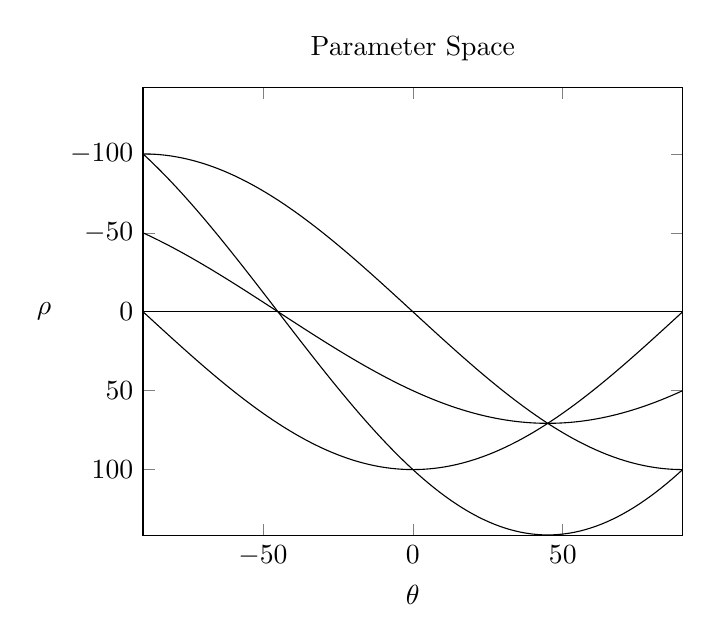
\begin{tikzpicture}
	\begin{axis}[title=Parameter Space, y dir=reverse, enlargelimits=false, ylabel=$\rho$,ylabel style={rotate=-90}, xlabel=$\theta$,xmin=-90,xmax=90,ymin=-142,ymax=142]
	\addplot[domain=-90:90, samples=101] {0* sin(x)};
	\addplot[domain=-90:90, samples=101] {100 * sin(x)};
	\addplot[domain=-90:90, samples=101] {70.7 * sin(x+45)};
	\addplot[domain=-90:90, samples=101] {100 * sin(x+90)};
	\addplot[domain=-90:90, samples=101] {141.4 * sin(x+45)};
	\end{axis}
	\end{tikzpicture}
\end{center}
(Realistically these sinusoids are just the patterns of the discrete bins, not actual sinusoidal curves, but I'm lazy and made 5 curves instead of $101^2$ boxes.) The locations where these curves intersect have accumulator values of 2 or 3 (however many curves intersect). From the intersection of the three curves at $(45, 70.7)$ and $(-45, 0)$, we conclude that there are three foreground points that lie on each lines diagonally across the image. Also notice how this special case of the Hough Transform is equivalent to the Radon Transform.

As a brief peek at generalization, the Hough Transform for a circle might be based on the parameterization
\begin{equation}
(x-a)^2 + (y-b)^2=r^2 \label{eq:hough:circle}
\end{equation}
where the center lies at $(a,b)$ with radius $r$. With three parameters, this algorithm is significantly more complex, though it can be decreased by knowing the radius of circle which is desired \textit{a priori}. Additionally, finding a circle presents interesting considerations, such as the \textit{center} of the circle not being within the original image space while the pixels that contribute to that circle do.
	
	\chapter{Computed Tomography: Physics and Reconstruction}
	\section{X-ray Summary}

\section{Rudimentary Projection Experiment Setup}

Radon Transform Equation

\begin{equation}
g(\rho_i,\theta_k) = \int_{-\infty}^{\infty} \int_{-\infty}^{\infty} I(x,y) \; \delta \big(xcos(\theta) + ysin(\theta) - \rho \big) \; dx \; dy
\label{eq:Radon}
\end{equation}

\noindent
where $g(\rho_i,\theta_k)$ is the radon transform for given sets $\{\rho_i\}$ and $\{\theta_k\}$, $I(x,y)$ is the image that is desired image, and $\delta$ is the dirac delta function. Back projection then uses these individual radon transforms to create a back-projected image.  For a given $\theta$ the back-projected image is the following:

\begin{equation}
f_{\theta}(x,y) = g(xcos(\theta) + ysin(\theta), \theta)
\end{equation}

\noindent
Summation of these individual back-projected images generates an image of the original object:

\begin{equation}
I(x,y) = \sum_{\theta=0}^{\pi} \: f_{\theta}(x,y) = \sum_{\theta=0}^{\pi} \: g(xcos(\theta) + ysin(\theta), \theta)
\end{equation}

Another method for reconstructing an image is to ust the central slice theorem which states that the 1-D Fourier transform of a radon transform is a single slice of the 2-D Fourier transform of the image that passes through the origin at angle $\theta$. To prove this, let us consider a single radon transform at angle $\theta$ and take the 1-D Fourier transform of it:

\begin{equation}
G(w,\theta) = \int_{-\infty}^{\infty} g(\rho,\theta) \: e^{i2\pi  w \rho} \: d\rho
\label{eq:1Dft}
\end{equation}

\noindent
substituting \ref{eq:Radon} into \ref{eq:1Dft} yeilds the following:

\begin{equation}
G(w,\theta) = \int_{-\infty}^{\infty} \: \biggl[  \int_{-\infty}^{\infty} \int_{-\infty}^{\infty} I(x,y) \; \delta \big(xcos(\theta) + ysin(\theta) - \rho \big) \; dx \; dy  \biggr] \: e^{i2\pi  w \rho} \: d\rho
\end{equation}

\noindent
rearranging this gives:

\begin{equation}
G(w,\theta) = \int_{-\infty}^{\infty} \int_{-\infty}^{\infty} I(x,y) \: \biggl[ \underbrace{ \int_{-\infty}^{\infty} \delta \big(xcos(\theta) + ysin(\theta) - \rho \big) e^{i2\pi w \rho} \: d\rho} \biggr] \: dx \: dy
\end{equation}

\noindent
using the properties of the dirac delta, the equation can be simplified:

\begin{equation}
G(w,\theta) = \int_{-\infty}^{\infty} \int_{-\infty}^{\infty} I(x,y)   e^{i2\pi w \big(xcos(\theta) + ysin(\theta) \big)} \: dx \: dy 
\end{equation}

\noindent
which is the 2-D Fourier transform along the line $wcos(\theta) + wsin(\theta)$


\section{Reconstruction from Projection Data}
	\part{Working}
	\chapter{Landmark Thin Plate Splines Registration}
	%11/10/15
	\chapter{Basic Diffeomorphic Image Registration}
	
	\chapter{Image de-noising/Wiener Filter}
	
	\chapter{Image mosaicking}
	
	\chapter{MRI image FOV calculation, Gx, Gy calculation}
	
	\chapter{Radial sampling, Gx, Gy, etc.}
	
	\chapter{Probability - Expected Value}
	
	\chapter{k-space - frequency and phase encoding}
	
	
	
	
	
	
		
\end{document}